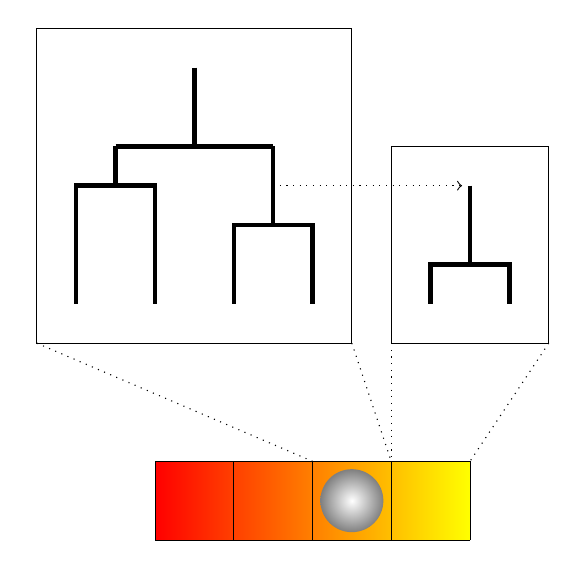
\begin{tikzpicture} 
  % Patch gradients
  \shade[left color=red,right color=yellow] (0,0) rectangle (4,1);
  % Species gradients
  \shade[inner color=white,outer color=gray] (2.5,0.5) circle (0.4 cm);
  % Grids
  \draw[step=1cm,black,very thin] (0,0) grid (4,1); 
  % Left species phylogeny
  \draw[] (-1.5,2.5) rectangle (2.5,6.5); 
  \draw[ultra thick] ( 0.5,6.0) node {} -- ( 0.5,5.0) node {}; 
  \draw[ultra thick] (-0.5,5.0) node {} -- ( 1.5,5.0) node {}; 
  \draw[ultra thick] (-0.5,5.0) node {} -- (-0.5,4.5) node {}; 
  \draw[ultra thick] ( 1.5,5.0) node {} -- ( 1.5,4.0) node {}; 
  \draw[ultra thick] (-1.0,3.0) node {} -- (-1.0,4.5) node {} -- ( 0.0,4.5) node {} -- ( 0.0,3.0) node {}; 
  \draw[ultra thick] ( 1.0,3.0) node {} -- ( 1.0,4.0) node {} -- ( 2.0,4.0) node {} -- ( 2.0,3.0) node {}; 
  % Right species phylogeny
  \draw[] ( 3.0,2.5) rectangle (5.0,5.0); 
  \draw[ultra thick] ( 4.0,4.5) node {} -- ( 4.0,3.5) node {}; 
  \draw[ultra thick] ( 3.5,3.0) node {} -- ( 3.5,3.5) node {} -- ( 4.5,3.5) node {} -- ( 4.5,3.0) node {}; 
  % Colonization line
  \draw[dotted,->] ( 1.5,4.5) node {} -- (4.0-0.1,4.5) node {}; 
  % Zoomers
  \draw[dotted] (-1.5,2.5) node {} -- (2,1) node {}; 
  \draw[dotted] ( 2.5,2.5) node {} -- (3,1) node {}; 
  \draw[dotted] ( 3.0,2.5) node {} -- (3,1) node {}; 
  \draw[dotted] ( 5.0,2.5) node {} -- (4,1) node {}; 
  
\end{tikzpicture}